% This file was created with tikzplotlib v0.10.1.
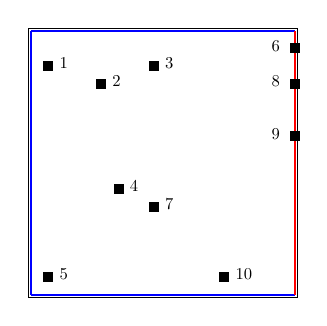
\begin{tikzpicture}

\begin{axis}[
% Set the aspect ratio to 1 for a square plot
unit vector ratio*=1 1 1,
% Set equal width and height
width=5cm,
height=5cm,
tick pos=left,
xmin=-0.01, xmax=1.01,
ymin=-0.01, ymax=1.01,
xtick=\empty, % remove xticks
ytick=\empty  % remove yticks
]
\addplot [thick, blue]
table {%
0 0
0 1
};
\addplot [thick, blue]
table {%
0 0
1 0
};
\addplot [thick, blue]
table {%
0 1
1 1
};
\addplot [thick, red]
table {%
1 0
1 1
};
\addplot [semithick, black, mark=square*, mark size=1.5, mark options={solid}, only marks]
table {%
0.0666666666666667 0.866666666666667
0.266666666666667 0.8
0.466666666666667 0.866666666666667
0.333333333333333 0.4
0.0666666666666667 0.0666666666666667
1 0.933333333333333
0.466666666666667 0.333333333333333
1 0.8
1 0.6
0.733333333333333 0.0666666666666667
};
\draw (axis cs:0.0866666666666667,0.856666666666667) node[
  scale=0.6,
  anchor=base west,
  text=black,
  rotate=0.0
]{1};
\draw (axis cs:0.286666666666667,0.79) node[
  scale=0.6,
  anchor=base west,
  text=black,
  rotate=0.0
]{2};
\draw (axis cs:0.486666666666667,0.856666666666667) node[
  scale=0.6,
  anchor=base west,
  text=black,
  rotate=0.0
]{3};
\draw (axis cs:0.353333333333333,0.39) node[
  scale=0.6,
  anchor=base west,
  text=black,
  rotate=0.0
]{4};
\draw (axis cs:0.0866666666666667,0.0566666666666667) node[
  scale=0.6,
  anchor=base west,
  text=black,
  rotate=0.0
]{5};
\draw (axis cs:0.89,0.923333333333333) node[
  scale=0.6,
  anchor=base west,
  text=black,
  rotate=0.0
]{6};
\draw (axis cs:0.486666666666667,0.323333333333333) node[
  scale=0.6,
  anchor=base west,
  text=black,
  rotate=0.0
]{7};
\draw (axis cs:0.89,0.79) node[
  scale=0.6,
  anchor=base west,
  text=black,
  rotate=0.0
]{8};
\draw (axis cs:0.89,0.59) node[
  scale=0.6,
  anchor=base west,
  text=black,
  rotate=0.0
]{9};
\draw (axis cs:0.753333333333333,0.0566666666666667) node[
  scale=0.6,
  anchor=base west,
  text=black,
  rotate=0.0
]{10};
\end{axis}

\end{tikzpicture}
